\documentclass{article}
\usepackage[a4paper,  hmargin=0.5in, vmargin=0.6in]{geometry}
\usepackage[utf8]{inputenc}
\usepackage{amsmath}
\usepackage{amsthm}
\usepackage{amsfonts}
\usepackage{bigints}
\usepackage{float}
\usepackage{svg}
\usepackage{multirow}
\usepackage[round]{natbib}
\usepackage{url}
\def\UrlBreaks{\do\/\do-}
\usepackage{breakurl}
\usepackage[hidelinks]{hyperref}
%\usepackage{layout}

\setlength{\topskip}{0mm}
\setlength{\parindent}{0mm}


\newcommand{\Et}{\mathbb{E}_t}
\newcommand{\E}{\mathcal{E}}

\title{\large{\textbf{Macroeconomics III - Project}} \\
\LARGE{Replication of New Keynesian Model for a Small Open Economy and Inclusion of Staggered Wages }
\author{Anna Catarina Batista Tavella\\Matheus Roberto de Bona Franciscão}}
\date{}

\begin{document}
\maketitle

\section*{Abstract}
This work first replicates the \cite{gali_monacelli} model for a small open economy. The model consists of a continuum of small economies that trade with each other. After the aggregation, the result is similar to a model of two countries: a small one, the domestic economy, and the rest of the world, which is not influenced by the domestic policies. As the model is based in monopolistic competition, to stabilize the output gap at zero in an efficient level, the authors considered a subsidy that guarantees the production in the efficient level (flexible prices). The authors analyse three types of monetary policy reaction: DITR (Domestic Inflation Taylor Rule), CITR (CPI Inflation Taylor Rule) and PEG (fixed exchange rate). Based on a welfare loss function, they found that the DITR has the best performance and the PEG has the worst. We then added wage rigidity to the model. With rigidity in two markets (goods market and labour market), it's not possible anymore to stabilize output gap, inflation of goods and inflation of wages at the same time (the choice is made to minimize the function loss). We also found that in this case, ranking of policy alternatives are inverted, with the PEG being the most effective and the DITR, the worst.

\section{Introduction}
Almost 100 years ago, Friedman stressed the importance of price changes (that is, inflation) and its correlation with business cycles in the USA. It may seem obvious that fiscal and monetary policies should be used to stabilize the economy, but the question is how. In our work, we restrict attention to monetary policy. \cite{friedman}, points out the mistakes done in the end of years 1920s by the recently created Federal Reserve (FED), that worsened the great depression. \cite{lucas}, develops a simple model to estimate the output-inflation trade-off in different countries. \cite{taylor_policy} examines empirical evidence of monetary policy rules, which is now known as "Taylor rule". As much of early work refers to US economy, in the subsequent years models were developed with interaction of countries, like \cite{gali_monacelli2002}. The \cite{gali_monacelli} paper arrives at the same equations for world output and inflation departing from a continuum of small open economies, which none of them alone can influence the world economy. Using this framework, the authors compare three monetary policy rules (domestic inflation target, CPI inflation target and exchange rate peg) with the optimal monetary policy. We extend this model to include sticky wages. \cite{rhee} included sticky prices, but also changed the openess parameter and added a parameter ($\phi_y$) for the output gap on the monetary policy rule. They found that the best policy rule depends on which model we consider for the analyzed economy.

\section{Description of the model}

\subsection{Consumers Problem}
The model considers a standard representative consumer with separable preferences who maximizes his expected discounted payoff in an infinite time horizon:
\begin{equation}
    \label{cons_problem}
    \max_{C_t, N_t} E_0 \sum^\infty_{t=0} \beta^t \left[\frac{C_t^{1-\sigma}}{1-\sigma} - \frac{N_t^{\varphi+1}}{\varphi+1} \right] \hspace{1em}  \textrm{ st. } \hspace{1em} \forall t, \hspace{0.8em} P_t C_t + \Et[Q_{t,t+1} D_{t+1}] \leq D_t +  W_t N_t + T_t
\end{equation}

where $D_t$ is the nominal payoff in period $t$ of the portfolio held at the end of period $t-1$. The consumer chooses between domestic goods ($C_{H,t}$) and foreign goods ($C_{F,t}$) with $\alpha \in [0,1]$ as the opening index of the economy and $\eta > 0$ as the elasticity of substitution between domestic and imported goods. The imported goods consists in a basket of goods imported from a continuum of different countries $i$ with elasticity of substitution $\gamma > 0$. Finally, he can choose between goods $j$ produced in the same country (domestic or foreign) with elasticity of substitution $\varepsilon > 0$.
\begin{equation}
    C_t \equiv \left[ (1-\alpha)^{\frac{1}{\eta}} (C_{H,t})^{\frac{\eta-1}{\eta}} + \alpha^{\frac{1}{\eta}} (C_{F,t})^{\frac{\eta-1}{\eta}} \right]^{\frac{\eta}{\eta-1}}
\end{equation}
\begin{subequations}
    \begin{minipage}{0.33\textwidth}
        \label{index_eqs}
        \begin{align}
            C_{F,t} \equiv \left( \int^1_0 C_{i,t}^{\frac{\gamma-1}{\gamma}} di \right)^{\frac{\gamma}{\gamma-1}} \label{foreign_index}
        \end{align}
    \end{minipage}
    \begin{minipage}{0.33\textwidth}
        \begin{align}
            C_{H,t} \equiv \left( \int^1_0 C_{H,t}(j)^{\frac{\varepsilon-1}{\varepsilon}} dj \right)^{\frac{\varepsilon}{\varepsilon-1}} \label{home_index}
        \end{align}
    \end{minipage}
    \begin{minipage}{0.33\textwidth}
        \begin{align}
            C_{i,t} \equiv \left( \int^1_0C_{i,t}(j)^{\frac{\varepsilon-1}{\varepsilon}} dj \right)^{\frac{\varepsilon}{\varepsilon-1}} \label{item_index}
        \end{align}
    \end{minipage}
\end{subequations}

The solution of the consumer's problem is detailed in the appendix A and results are, as usual, the consumer Euler equation and the labor supply, with $W_t^R$ as the real wage. 

\vspace{6pt}

\begin{minipage}{0.49\textwidth}
    \begin{equation}
        \label{euler}
        \beta R_t \Et\left[\left(\frac{C_{t+1}}{C_t} \right)^{-\sigma} \left(\frac{P_t}{P_{t+1}} \right) \right] = 1
    \end{equation}
\end{minipage}
\begin{minipage}{0.49\textwidth}
    \begin{equation}
        \label{labour_supply}
        C_t^\sigma N_t^\varphi = \frac{W_t}{P_t} \equiv W_t^R
    \end{equation}
\end{minipage}

\vspace{6pt}
We get also the and the demand functions and the proportion of domestic and imported goods:

\begin{subequations}
    \begin{minipage}{0.33\textwidth}
        \label{demand_eqs}
        \begin{align}
            C_{H,t}(j) = \left( {\frac{P_{H,t}(j)}{P_{H,t}}} \right)^{-\varepsilon}C_{H,t} \label{Chj_demand}
        \end{align}
    \end{minipage}
    \begin{minipage}{0.33\textwidth}
        \begin{align}
            C_{i,t}(j) = \left( {\frac{P_{i,t}(j)}{P_{i,t}}} \right)^{-\varepsilon}C_{i,t} \label{Cij_demand}
        \end{align}
    \end{minipage}
    \begin{minipage}{0.33\textwidth}
        \begin{align}
            C_{i,t} = \left( {\frac{P_{i,t}}{P_{F,t}}} \right)^{-\gamma}C_{F,t}\label{Ci_demand}
        \end{align}
    \end{minipage}
\end{subequations}

\begin{subequations}
    \begin{minipage}{0.33\textwidth}
        \label{Cf_demand}
        \begin{align}
            C_{F,t} = \alpha \left( \frac{P_{F,t}}{P_t} \right)^{-\eta}C_t
        \end{align}
    \end{minipage}
    \begin{minipage}{0.33\textwidth}
        \label{Ch_demand}
        \begin{align}
            C_{H,t} = (1-\alpha)\left( \frac{P_{H,t}}{P_t} \right)^{-\eta}C_t
        \end{align}
\end{minipage}
\end{subequations}

\subsection{Terms of trade}
We define the bilateral terms of trade $S_{i,t}$ between domestic economy and the country $i$ as $S_{i,t} \equiv \frac{P_{i,t}}{P_{H,t}}$. The effective terms of trade is given by:
\begin{equation}
    S_t \equiv \left(\int^1_0 S_{i,t}^{1-\gamma} di \right)^{\frac{1}{1-\gamma}} = \left(\int^1_0 \left(\frac{P_{i,t}}{P_{H,t}}  \right)^{1-\gamma}  di \right)^{\frac{1}{1-\gamma}} = \frac{1}{P_{H,t}} \left(\int^1_0 \left(P_{i,t}^{1-\gamma} di \right)^{\frac{1}{1-\gamma}}\right) = \frac{P_{F,t}}{P_{H,t}}
\end{equation}

Using the fact that price level is given by $P_t^{1-\eta} = (1-\alpha) P_{H,t}^{1-\eta} + \alpha P_{F,t}^{1-\eta}$ we get:
\begin{equation}
    \label{tot_level}
    P_t^{1-\eta} = (1-\alpha) P_{H,t}^{1-\eta} + \alpha \left( P_{H,t}^{1-\eta} S_{t}^{1-\eta} \right) = P_{H,t}^{1-\eta} \left[(1-\alpha) + \alpha S_t^{1-\eta} \right] \Rightarrow P_t = P_{H,t} \left[(1-\alpha) + \alpha S_t^{1-\eta} \right]^{\frac{1}{1-\eta}} 
\end{equation}

Dividing both sides by $P_{t-1}$:
\begin{equation}
    \label{tot}
    \frac{P_t}{P_{t-1}} = \frac{P_{H,t} \left[(1-\alpha) + \alpha S_t^{1-\eta} \right]^{\frac{1}{1-\eta}}} {P_{H,t-1} \left[(1-\alpha) + \alpha S_{t-1}^{1-\eta} \right]^{\frac{1}{1-\eta}}} \Rightarrow \Pi_t = \Pi_{H,t} \left(\frac{(1-\alpha) + \alpha S_t^{1-\eta}} {(1-\alpha) + \alpha S_{t-1}^{1-\eta}} \right)^{\frac{1}{1-\eta}}
\end{equation}

\subsection{Exchange Rate}
We assume that law of one price holds for all goods at all times, defining $\E_{i,t}$ as the bilateral exchange rate between domestic economy and country $i$ and $P^i_{i,t}(j)$ as the price expressed in the producer's currency, then:
\begin{equation}
    P_{i,t}(j) = \E_{i,t} P^i_{i,t}(j) \Rightarrow \left( \int^1_0 \left(P_{i,t}(j) \right)^{1-\epsilon} dj \right)^{\frac{1}{1-\epsilon}} = \left( \int^1_0 \left(\E_{i,t} P^i_{i,t}(j) \right)^{1-\epsilon} dj \right)^{\frac{1}{1-\epsilon}} \Rightarrow P_{i,t} = \E_{i,t} P^i_{i,t}
\end{equation}

Aggregating for all countries $i$
\begin{equation}
    \left( \int^1_0 \left(P_{i,t} \right)^{1-\gamma} di \right)^{\frac{1}{1-\gamma}} = \left( \int^1_0 \left(\E_{i,t} P^i_{i,t} \right)^{1-\gamma} di \right)^{\frac{1}{1-\gamma}} \Rightarrow S_t P_{H,t} = \left( \int^1_0 \left(\E_{i,t} P^i_{i,t} \right)^{1-\gamma} di \right)^{\frac{1}{1-\gamma}}
\end{equation}

Dividing $S_t P_{H,t}$ by $S_{t-1} P_{H,t-1}$ and using the same expression for the period $t-1$, we get:
\begin{equation}
    \label{fx}
    \frac{S_t P_{H,t}}{S_{t-1} P_{H,t-1}} = \frac{\left( \int^1_0 \left(\E_{i,t} P^i_{i,t} \right)^{1-\gamma} di \right)^{\frac{1}{1-\gamma}}}{\left( \int^1_0 \left(\E_{i,t-1} P^i_{i,t-1} \right)^{1-\gamma} di \right)^{\frac{1}{1-\gamma}}} \Rightarrow \frac{S_t}{S_{t-1}}\Pi_{H,t} = \left(\frac{\int^1_0 \left(\E_{i,t} P^i_{i,t} \right)^{1-\gamma} di }{\int^1_0 \left(\E_{i,t-1} P^i_{i,t-1} \right)^{1-\gamma} di} \right)^{\frac{1}{1-\gamma}}
\end{equation}

which defines implicitly $\E_{t} \equiv \left( \int^1_0 \E_{i,t}^{\frac{\gamma-1}{\gamma}} di \right)^{\frac{\gamma}{\gamma-1}}$ as the nominal effective exchange rate \footnote{Log-linearizing we get $\pi_{H,t+1} + s_{t+1} - s_t = \pi^*_{t+1} + \Delta e_{t+1}$, where $e_t \equiv \int^1_0 e_{i,t}$, $p_t^* \equiv \int^1_0 p^i_{i,t}$ and $\pi^*_t \equiv p_t^* - p_{t-1}^*$. The baseline model of the paper assumes $p_t^* = p^* = 0$, implying that $\pi_{H,t+1} + s_{t+1} - s_t = \Delta e_{t+1}$}.

The bilateral real exchange rate with country $i$ is defined as $\mathcal{Q}_{i,t} \equiv \frac{\E_{i,t} P^i_{i,t}}{P_t}$ and using that $P_{i,t} = \E_{i,t} P^i_{i,t}$ then:
\begin{equation}
\label{real_rate}
\begin{split}
\mathcal{Q}_{i,t} & = \frac{\E_{i,t} P^i_{i,t}}{P_t} = \frac{P_{i,t}}{P_t} \Rightarrow \left( \int^1_0 \mathcal Q_{i,t}^{1-\gamma} di \right)^{\frac{1}{1-\gamma}} = \left( \int^1_0 \left(\frac{P_{i,t}}{P_t}\right)^{1-\gamma} di \right)^{\frac{1}{1-\gamma}} = \frac{1}{P_t}\left( \int^1_0 P_{i,t}^{1-\gamma} di \right)^{\frac{1}{1-\gamma}} \\
\mathcal{Q}_{t} & = \frac{P_{F,t}}{P_t} = \frac{P_{H,t} S_t}{P_t} = \frac{P_{H,t} S_t}{P_{H,t} \left[(1-\alpha) + \alpha S_t^{1-\eta} \right]^{\frac{1}{1-\eta}}} = \left[(1-\alpha)S_t^{\eta-1} + \alpha \right]^{\frac{1}{\eta-1}}
\end{split}
\end{equation}
\vspace{6pt}
\subsection{Firms Problem}

A representative firm has a technology with constant returns to scale:
\begin{equation}
    \label{technology}
    Y_t(j) = A_t N_t(j) \Rightarrow \int^1_0 Y_t(j) dj = \int^1_0 A_t N_t(j) dj \Rightarrow \int^1_0 Y_t(j) dj = A_t N_t 
\end{equation}

\begin{equation}
    \label{tfp}
    A_{t+1} = {A_t}^{\rho_a}\exp( \varepsilon^a_t)
\end{equation}

where $A_t$ is such that $a_t \equiv \ln(A_t)$ follows an AR(1) process and in steady state we normalize $A = 1$.

\vspace{6pt}

The model assumes sticky prices following Calvo (1983): at each period a random selected fraction $\theta$ of firms have to keep their prices unchanged from the previous period, while the remaining $1-\theta$ firms can reset them. If a firm can adjust its price at time $t$, we set its price at $\overline{p}_{H,t}$ which maximizes the present value of its future profits:
\begin{equation}
    \overline{p}_{H,t} = \max_{\overline{p}_{H,t}} \sum^\infty_{k=0} \theta^k \Et \left[ Q_{t, t+k}[Y_{t+k}(j) (\overline{p}_{H,t} - MC_{t+k} P_{H,t+k})] \right]
\end{equation}

where $MC_t$ is the real marginal cost. Combining the first order of this problem with the price dynamics (detailed solution is in appendix B) and defining $\widehat{MC}_t = \frac{MC_t}{1/ \mathcal M}$ as the marginal cost deviation from steady state we get:
\begin{equation}
    \label{nkpc}
    \Pi_{H,t} = \left[ \theta + \frac{(1-\theta)}{P_{H,t-1}^{1-\varepsilon}} \left(\frac{\Et\left[ \sum^\infty_{k=0} (\beta\theta)^k C_{t+k}^{-\sigma} \frac{1}{P_{t+k}}\widetilde C_{H,t+k} P_{H,t+k} \widehat{MC}_{t+k}\right] }{\Et\left[ \sum^\infty_{k=0} (\beta\theta)^k C_{t+k}^{-\sigma} \frac{1}{P_{t+k}} \widetilde C_{H,t+k}  \right]} \right)^{1-\varepsilon}\right]^\frac{1}{1-\varepsilon}
\end{equation}

Finally, due to constant returns to scale, the real marginal cost does not depend on quantities. Using the consumers labor supply (\ref{labour_supply}), the technology (\ref{technology}) and (\ref{tot_level}) we can derive the marginal cost deviation from its steady state:
\begin{equation}
    \label{marginal_cost}
    \widehat{MC}_t = \mathcal M MC_t = \frac{W_t (1 - \tau) \mathcal M}{P_{H,t}A_t} = \frac{W_t P_t (1 - \tau)\mathcal M}{P_t P_{H,t}A_t}
    = \frac{W_t^R \left[(1-\alpha) + \alpha S_t^{1-\eta} \right]^{\frac{1}{1-\eta}} (1 - \tau) \mathcal M}{A_t^{1+\varphi}}
\end{equation}
where $\tau$ is an employment subsidy \footnote{See appendix C for discussion on optimal subsidy} and $\frac{W_t}{P_{H,t}}$ is the real wage in the firm's perspective\footnote{On consumer problem's the real wage $W_t^R \equiv \frac{W_t}{P_t}$ was defined considering the total price index, however when calculating the real marginal cost of the domestic firms the paper uses the real wage considering only the domestic price index $\left( \frac{W_t}{P_{H,t}}\right)$ . This is consistent with no mobility of workers between countries}.

\vspace{6pt}

\subsection{Rest of the world}
Given the small domestic economy, we assume that the rest of the world's output $Y_t^*$ can be taken as exogenous and such that $y_t^* = \ln(Y^*_t)$ follows and AR(1) process:
\begin{equation}
    \label{y_row}
    Y^*_{t+1} = {Y^*_t}^{\rho_y}\exp( \varepsilon^*_t)
\end{equation}

Consumer's Euler equations also holds for a representative consumer in any other country:

$$\beta \left( \frac{C^i_{t+1}}{C_t^i} \right) \left( \frac{P_t^i}{P^i_{t+1}} \right) \left( \frac{\E^i_t}{\E^i_{t+1}} \right) = Q^i_{t, t+1}$$

The model assumes complete markets, thus, there are perfect domestic and international risk sharing, implying that $Q^i_{t, t+1} = Q_{t,t+1}$:
\begin{equation}
\begin{array}{cc}
     &\displaystyle \beta \left( \frac{C^i_{t+1}}{C_t^i} \right)^{-\sigma} \left( \frac{P_t^i \E^i_t}{P^i_{t+1} \E^i_{t+1}} \right) = \beta \left( \frac{C_{t+1}}{C_t^i} \right)^{-\sigma} \left( \frac{P_t}{P_{t+1}} \right) \Rightarrow \left( \frac{C_{t+1}}{C_t^i} \right) = \left( \frac{C^i_{t+1}}{C_t^i} \right) \left(\frac{\frac{\E_{i,t+1} P^i_{t+1}}{P_{t+1}}}{\frac{\E_{i,t} P^i_{t}}{P_{t}}} \right)^{\frac{1}{\sigma}} \\
     & \displaystyle \left( \frac{C_{t+1}}{C_t} \right) = \left( \frac{C^i_{t+1}}{C_t^i} \right) \left(\frac{\mathcal{Q}_{i,t+1}}{\mathcal{Q}_{i,t}} \right)^{\frac{1}{\sigma}} \Rightarrow \left[\frac{C_{t+1}}{C^i_{t+1} \mathcal Q_{i,t+1}^{\frac{1}{\sigma}}}\right] =  \left[\frac{C_t}{C^i_t \mathcal Q_{i,t}^{\frac{1}{\sigma}}} \right] \\
\end{array}
\end{equation}

Defining $t = 0$ and iterating we get that, for all period $t$
\begin{equation}
    \label{riskSharing}
    \left[\frac{C_{t}}{C^i_{t} \mathcal Q_{i,t}^{\frac{1}{\sigma}}}\right] =  \left[\frac{C_0}{C^i_0 \mathcal Q_{i,0}^{\frac{1}{\sigma}}} \right] \equiv v_{i, 0} \Rightarrow C_t = v_{i,0} C^i_t \mathcal Q_{i,t}^{\frac{1}{\sigma}}
\end{equation}

where $v_{i,0}$ depends on initial conditions, which the model assumes to be symmetric, then $v_{i,0} = 1$ for all $i$. Aggregating over all countries:
\begin{equation}
    \label{consumption}
    \left(\int^1_0 C_t^{1-\gamma} di \right)^{\frac{1}{1-\gamma}} \equiv C_t = \left(\int^1_0  \left(C_t^i \mathcal Q_{i,t}^{\frac{1}{\sigma}}\right)^{1-\gamma} di \right)^{\frac{1}{1-\gamma}}
\end{equation}

\subsection{Market clearing}
For each domestic good, the total production is equal to domestic + external demands. Substituting the expressions obtained in the consumer problem and aggregating for all domestic goods (detailed steps are in appendix D) we obtain:
\begin{equation}
    \label{output_st}
    Y_{t} = C_t \left[(1-\alpha) + \alpha S_t^{1-\eta} \right]^{\frac{\eta}{1-\eta}} \left[(1-\alpha)  +  \alpha \int_0^1 \left(\mathcal S^i_t \mathcal S_{i,t} \right)^{\gamma - \eta} \mathcal Q^{\eta - \frac{1}{\sigma}}_{i,t} di \right] 
\end{equation}

As we are considering the country as a small open economy: for the rest of the world, the domestic consumption and production are insignificant and can be ignored, so market clearing implies:
\begin{equation}
    \label{world_equilibrium}
    C_t^* = Y_t^*
\end{equation}

\section{Equilibrium conditions}
The equilibrium conditions (without a monetary policy equation) are given by equations (\ref{euler}), (\ref{labour_supply}), (\ref{tot}), (\ref{fx}), (\ref{real_rate}), (\ref{technology}), (\ref{tfp}), (\ref{marginal_cost}), (\ref{nkpc}), (\ref{y_row}), (\ref{consumption}), (\ref{output_st}) and (\ref{world_equilibrium}) obtained above:

\begin{subequations}
    \label{se}
    \begin{minipage}{0.5\textwidth}
        \begin{align}
            &\beta R_t \Et\left[\left(\frac{C_{t+1}}{C_t} \right)^{-\sigma} \left(\frac{P_t}{P_{t+1}} \right) \right] = 1 \label{euler_eq}\\
            & C_t^\sigma N_t^\varphi = W_t^R \label{labour_supply_eq}\\
            &\Pi_t = \Pi_{H,t} \left(\frac{(1-\alpha) + \alpha S_t^{1-\eta}} {(1-\alpha) + \alpha S_{t-1}^{1-\eta}} \right)^{\frac{1}{1-\eta}} \label{tot_eq}\\
            &\frac{S_t}{S_{t-1}}\Pi_{H,t} = \left(\frac{\int^1_0 \left(\E_{i,t} P^i_{i,t} \right)^{1-\gamma} di }{\int^1_0 \left(\E_{i,t-1} P^i_{i,t-1} \right)^{1-\gamma} di} \right)^{\frac{1}{1-\gamma}} \label{fx_eq}
        \end{align}
    \end{minipage}
    \begin{minipage}{0.5\textwidth}
        \begin{align}
            &\mathcal{Q}_{t}  = \left[(1-\alpha)S_t^{\eta-1} + \alpha \right]^{\frac{1}{\eta-1}} \label{real_rate_eq}\\
            &\int^1_0 Y_t(j) dj = A_t N_t \label{technology_eq}\\
            &A_{t+1} = {A_t}^{\rho_a}\exp( \varepsilon^a_{t+1}) \label{tfp_eq}\\
            &\widehat{MC}_t  = \frac{W_t^R \left[(1-\alpha) + \alpha S_t^{1-\eta} \right]^{\frac{1}{1-\eta}} (1 - \tau) \mathcal M}{A_t^{1+\varphi}} \label{marginal_cost_eq}\\
        \end{align}
    \end{minipage}
    \begin{align}
        &\Pi_{H,t} = \left[ \theta + \frac{(1-\theta)}{P_{H,t-1}^{1-\varepsilon}} \left(\frac{\Et\left[ \sum^\infty_{k=0} (\beta\theta)^k C_{t+k}^{-\sigma} \frac{1}{P_{t+k}}\tilde C_{H,t+k} P_{H,t+k} \widehat{MC}_{t+k}\right] }{\Et\left[ \sum^\infty_{k=0} (\beta\theta)^k C_{t+k}^{-\sigma} \frac{1}{P_{t+k}} \tilde C_{H,t+k}  \right]} \right)^{1-\varepsilon}\right]^\frac{1}{1-\varepsilon} \label{nkpc_eq}\\
        &Y^*_{t+1} = {Y^*_t}^{\rho_y}\exp( \varepsilon^*_{t+1}) \label{y_row_eq}\\
        &C_t = \left(\int^1_0  \left(C_t^i \mathcal Q_{i,t}^{\frac{1}{\sigma}}\right)^{1-\gamma} di \right)^{\frac{1}{1-\gamma}} \label{consumption_eq}\\
        &Y_{t} = C_t \left[(1-\alpha) + \alpha S_t^{1-\eta} \right]^{\frac{\eta}{1-\eta}} \left[(1-\alpha)  +  \alpha \int_0^1 \left(\mathcal S^i_t \mathcal S_{i,t} \right)^{\gamma - \eta} \mathcal Q^{\eta - \frac{1}{\sigma}}_{i,t} di \right] \label{output_st_eq}\\
        & C_t^* = Y_t^* \label{world_equilibrium_eq}
    \end{align}
\end{subequations}

The equations resulting of the first-order linear approximation around the steady state \footnote{The order of log-linearized equation was chosen to match the code. The (transposed) vector of endogenous variables in the code is $[x_t, y_t^*, \pi_{H,t}, a_t, r_t, \overline{y}_t, y_t, c_t^*, s_t, q_t, c_t, \pi_t, \Delta e_t, \widehat{mc}_t, n_t, w_t^R]$} from (\ref{euler_eq}), (\ref{nkpc_eq}), (\ref{tfp_eq}), (\ref{y_row_eq}), (\ref{world_equilibrium_eq}), (\ref{consumption_eq}), (\ref{real_rate_eq}), (\ref{output_st_eq}), (\ref{fx_eq}), (\ref{tot_eq}), (\ref{marginal_cost_eq}) (\ref{technology_eq}) and (\ref{labour_supply_eq}) are \footnote{Lower case letters represent the neperian logarithm of the original variables. We define $\rho \equiv \beta^{-1} -1$,  $\nu \equiv -ln(1-\tau)$, $\mu \equiv \ln(\mathcal M)$, $\omega \equiv \sigma \gamma + (1-\alpha)(\sigma \eta - 1)$, $\sigma_\alpha \equiv \frac{\sigma}{(1-\alpha) + \alpha \omega}$, $\Omega \equiv \frac{\nu - \mu}{\sigma_\alpha + \varphi}$, $\Gamma \equiv \frac{1 + \varphi}{\sigma_\alpha + \varphi}$, $\Psi \equiv \frac{(1-\omega) \alpha}{\sigma_\alpha + \varphi}$}:

\begin{subequations}
\label{sistema_loglin}
    \begin{minipage}{0.49\textwidth}
        \begin{align}
            &c_t = \Et[c_{t+1}] - \frac{1}{\sigma} (r_t - \Et[\pi_{t+1}] - \rho) \label{euler_log}\\
            & \pi_{H,t} = \beta \Et[\pi_{H,t+1}] + \lambda \widehat{mc}_t \label{nkpc_log}\\
            & \text{Monetary policy rule}\\
            &a_{t+1} = \rho_a a_t + \varepsilon^a_{t+1} \label{tfp_log}\\
            &y^*_{t+1} = \rho_y y^*_t + \varepsilon^*_{t+1} \label{y_row_log}\\
            &\overline{y}_t = \Omega + \Gamma a_t + \alpha \Psi y_t^* \label{y_bar_log}\\
            &x_t = y_t - \overline{y}_t \label{output_gap_log}\\
            &c_t^* = y_t^* \label{world_equilibrium_log}
        \end{align}
        \end{minipage}
        \begin{minipage}{0.49\textwidth}
        \begin{align}
            &c_t = c_t^* + \frac{1}{\sigma} q_t \label{consumption_log}\\
            &q_t = (1-\alpha) s_t \label{real_rate_log}\\
            &y_t = c_t + \alpha \gamma s_t + \alpha \left( \eta - \frac{1}{\sigma} \right) q_t \label{output_st_log}\\
            &\pi_t = \pi_{H,t} + \alpha s_t - \alpha s_{t-1} \label{tot_log}\\
            &s_{t} - s_{t-1} + \pi_{H,t} = \Delta e_t \label{fx_log}\\
            &\widehat{mc}_{t} = -\nu + \mu + w_t^R + \alpha s_t - a_t \label{marginal_cost_log}\\
            &y_t = a_t +  n_t \label{technology_log}\\
            & w_t^R = \sigma c_t + \varphi n_t \label{labour_supply_log}
        \end{align}
    \end{minipage}
\end{subequations}

\vspace{6pt}
To the log-linearized system (equations \ref{se}) we also add (\ref{y_bar_log}), a definition of potential output $\overline{y}_t$ obtained from (\ref{marginal_cost_log}) when $\widehat{mc}_t = 0$ and manipulating to be a function only of exogenous variables; and (\ref{output_gap_log}), a definition of (log) output gap given by output deviation from its potential. 

\vspace{6pt}

The paper suggests 3 different monetary rules and an optimal monetary rule benchmark\footnote{See appendix E for details} and estimates the model in each case:

\begin{itemize}
    \item Optimal Monetary Policy: $r_t = \overline{rr}_t + \phi_\pi \pi_{H, t}$
    \item Domestic Inflation Taylor Rule: $r_t = \rho + \phi_\pi \pi_{H, t}$
    \item CPI Inflation Taylor Rule: $r_t = \rho + \phi_\pi \pi_{t}$
    \item Exchange Rate Peg\footnote{The paper defines Peg as $e_t = 0$ but as the nominal variables are not determined in equilibrium, depending on the initial conditions (only their variations like inflation rates and $\Delta e_t$ are determined) we considered peg as $\Delta e_t = 0$, imposing an initial condition $e_0 = 0$ which implies in $e_t = 0$.}: $\Delta e_t = 0$.
\end{itemize}

Where $\overline{rr}_t = \rho + \sigma_\alpha \Gamma (1 - \rho_a) a_t + \alpha \sigma_\alpha (\Theta + \Psi)(\Et[y_{t+1}^*] - y_t^*)$ is the natural interest rate.

\section{Calibration}
The paper assumes the following calibration for the structural parameters:

\begin{minipage}{0.76\textwidth}
    \begin{table}[H]
        \centering
        \begin{tabular}{clc}
            \hline
            \textbf{Parameter} & \textbf{Description} & \textbf{Value}\\
            \hline
            \multicolumn{3}{l}{\textit{Common to Real Business Cycles Model}}\\
            $\beta$ & Intertemporal discount factor & $0.99$\\
            $\sigma$ & Inverse elasticity of intertemporal subsititution & $1$\\
            $\varphi$ & Inverse Frisch elasticity of labour supply & $3$\\
            $\rho_a$ & Productivity shock smoothing & $0.66$\\
            $\sigma_a$ & Standard deviation of the productivity shocks & $0.0071$ \\
            \multicolumn{3}{l}{\textit{Common to New Keynesian Model}}\\
            $\varepsilon$ & Substitutability between varieties (from the same country) & $6$\\
            $\theta$ & Calvo price stickiness & $0.75$\\
            $\phi_\pi$ & Taylor rule response to inflation & $1.5$ \\
            \multicolumn{3}{l}{\textit{Specific to Galí and Monacelli Model}}\\
            $\alpha$ & Opening index of the economy  & $0.4$\\
            $\eta$ & Substitutability between domestic and imported goods & $1$\\
            $\gamma$ & Substitutability between goods from different foreign countries & $1$\\
            $\rho_{y^*}$ & World GDP shock smoothing & $0.86$\\
            $\sigma_{y^*}$ & Standard deviation of the world GDP shocks & $0.0078$ \\
            $\rho_{ay^*}$ & Correlation between prod. and world GDP shocks & $0.3$ \\
            \hline
        \end{tabular}
    \end{table}
\end{minipage}
\begin{minipage}{0.23\textwidth}
    The values were calibrated with data from Canada, the small economy used as prototype by the authors. In the paper's text and tables the parameter $\rho_a$ is defined as $0.66$, however the IRFs charts are compatible with value $\rho_a = 0.90$ (apparently authors reused the charts from an working paper version \citep{gali_monacelli2002} without updating the figure or informed a different parameter in the text). We use $\rho_a = 0.90$ in the charts to be comparable with original ones in the paper. However, the other calculations are done with $\rho_a = 0.66$.
\end{minipage}

\section{Steady State Properties}
In the steady state: (i) Purchasing Power Parity holds symmetrically for all other countries (then $\mathcal Q_i = \mathcal Q$, $S_i = S$, $S^i=1$ and $C^i = C^*$), (ii) all the stationary variables are constant and (iii) there is not uncertainty ($\varepsilon^* = \varepsilon^a = 0$).  Using the equilibrium conditions showed in (\ref{se}) immediately by (g), (j) and (m) we obtain that $A = Y^* = C^* = 1$. The equation (a) defines $R = \beta^{-1}$. From (d) and (c) we have $\Pi = \Pi_H = 1$. Using (i) we find $\widehat{MC} = 1$. The remaining system (composed by equations (b), (e), (f), (l) and (l)) is:

\begin{subequations}
    \label{ser}
    \begin{minipage}{0.4\textwidth}
        \begin{align}
            & C^\sigma N^\varphi = W^R \\
            &\mathcal{Q} = \left[(1-\alpha)S^{\eta-1} + \alpha \right]^{\frac{1}{\eta-1}}\\
            &Y =  N
        \end{align}
    \end{minipage}
    \begin{minipage}{0.59\textwidth}
        \begin{align}
            &1 = W^R \left[(1-\alpha) + \alpha S^{1-\eta} \right]^{\frac{1}{1-\eta}} (1 - \tau) \mathcal M\\
            &C = \mathcal Q^{\frac{1}{\sigma}}\\
            &Y = C \left[(1-\alpha) + \alpha S^{1-\eta} \right]^{\frac{\eta}{1-\eta}} \left[(1-\alpha)  +  \alpha \mathcal S^{\gamma - \eta} \mathcal Q^{\eta - \frac{1}{\sigma}} \right]
        \end{align}
    \end{minipage}
\end{subequations}

\vspace{6pt}

This system cannot be solved analytically in the general case, however, using the values showed in calibration for $\alpha, \sigma, \eta, \gamma, \varepsilon$ and $\varphi$ and defining the optimal subsidy ($ 1-\tau = \frac{1}{(1-\alpha)\mathcal M}  $), as showed in appendix C, we obtain the following steady state values:

\begin{minipage}{0.59\textwidth}
    \begin{table}[H]
        \centering
        \begin{tabular}{clc}
            \hline
            \textbf{Variable} & \textbf{Description} & \textbf{Value}\\
            \hline
            $Y$ & Output & 1.13622 \\
            $C$ & Consumption & 1.07964 \\
            $W^R$ & Real wage & 1.58367 \\
            $C/Y$ & Consumption-to-GDP Ratio & 0.95020 \\
            $S$ & Terms of trade & 1.13622 \\
            $NX/Y$ & New exports in terms of domestic output & $0.00000$\\
            $(R^4 -1)$ & Real annual interest rate &  0.04102\\
            \hline
        \end{tabular}
    \end{table}
\end{minipage}
\begin{minipage}{0.40\textwidth}
    Our approach to calculate the steady-state considers that the small economy has incentives to adopt the optimal subsidy and benefit with the better terms of trade. This condition is imposed after the aggregation, otherwise if all the small economies had the same subsidy the steady-state would be symmetric ($S^i = S_i = S = 1$) and its value would be $1-\tau = \frac{1}{\mathcal M}$.
\end{minipage}

Note that consumption-to-GDP ratio is lower than 1 while net exports is zero, showing an apparent contradiction. However it is justified as domestic output and domestic consumption uses different prices indexes ($P_H$ and $P$, respectively), then net exports in terms of domestic output is given by $\frac{NX}{Y} = \frac{(Y - C \frac{P}{P_H})}{Y} = 1 - \frac{C}{Y} \frac{P}{P_H} = 1 - \frac{C}{Y} S^{0.4} = 0 $.

\section{Dynamic Properties}

\begin{minipage}{0.50\textwidth}
    Simulating 1000 samples with 201 periods each we obtained the following dynamic properties:
    \begin{table}[H]
        \centering
        \begin{tabular}{lcccc}
            \hline
            & Optimal & DITR & CITR & Peg\\
            & sd\% & sd\% & sd\% & sd\% \\
            \hline
            Output & 0.93 & 0.66 & 0.70 & 0.84 \\
            Domestic inflation & 0.00 & 0.27 & 0.26 & 0.35 \\
            CPI inflation & 0.38 & 0.40 & 0.26 & 0.21 \\
            Nominal int. rate & 0.32 & 0.40 & 0.40 & 0.21 \\
            Terms of trade & 1.52 & 1.43 & 1.33 & 1.08 \\
            Nominal depr. rate & 0.95 & 0.85 & 0.52 & 0.00 \\
            \hline
            \multicolumn{5}{l}{\textit{Note: } Sd denotes standard deviation in \%}
        \end{tabular}
    \end{table}
    It's interesting to note that even with different measures of $\mu$ (markup) and $\varphi$, comparing results from CPI inflation and domestic inflation the conclusion is that the results are quite similar in both cases. On the other hand, when comparing the inflation target with peg, when the peg is chosen the output gap is three times as volatile and the domestic inflation is almost twice as volatile, what makes the households worse off. In the next section the difference between the policies will be more evident.
\end{minipage}
\begin{minipage}{0.02\textwidth}
\end{minipage}
\begin{minipage}{0.47\textwidth}
    The contribution to welfare losses are:
    \begin{table}[H]
        \centering
        \begin{tabular}{lcccc}
            \hline
            &  DI Taylor & CPI Taylor & Peg\\
            \hline
            \multicolumn{4}{c}{Benchmark $\mu = 1.2$, $\varphi = 3$}\\
            Var(Domestic infl.) & 0.0150 & 0.0143 & 0.0259 \\
            Var(Output gap) & 0.0009 & 0.0019 & 0.0052 \\
            Total & 0.0159 & 0.0162 & 0.0311 \\
            \multicolumn{4}{c}{Low steady state markup $\mu = 1.1$, $\varphi = 3$}\\
            Var(Domestic infl.) & 0.0277 & 0.0262 & 0.0472 \\
            Var(Output gap) & 0.0009 & 0.0019 & 0.0052 \\
            Total & 0.0287 & 0.0281 & 0.0524 \\
            \multicolumn{4}{c}{Low elasticity of labour supply $\mu = 1.2$, $\varphi = 10$}\\
            Var(Domestic infl.) & 0.0226 & 0.0230 & 0.0556 \\
            Var(Output gap) & 0.0005 & 0.0020 & 0.0064 \\
            Total & 0.0231 & 0.0250 & 0.0620 \\
            \multicolumn{4}{c}{Low markup and elast. of labour supply $\mu = 1.1$, $\varphi = 10$}\\
            Var(Domestic infl.) & 0.0415 & 0.0421 & 0.1011 \\
            Var(Output gap) & 0.0005 & 0.0020 & 0.0063 \\
            Total & 0.0420 & 0.0440 & 0.1074 \\
            \hline
            \multicolumn{4}{l}{\textit{Note: } Values are \% units of steady state consumption}
        \end{tabular}
    \end{table}
\end{minipage}

\section{Impulse Response Functions}

\subsection{TFP shock}
We show the IRFs relative to an AR(1) productivity shock, as in the original paper. The shock hits only the analyzed economy and is the same for all policy rules adopted. It's important to notice that in this kind of model the monetary authority reacts immediately, the economy responds immediately, (activity and prices) and interest rates are allowed to be set below zero (i.e., there's no zero lower bound limitation). Also, the output gap is defined relative to the contrafactual with flexible prices, which fluctuates with the productivity.

\begin{figure}[H]
\centering
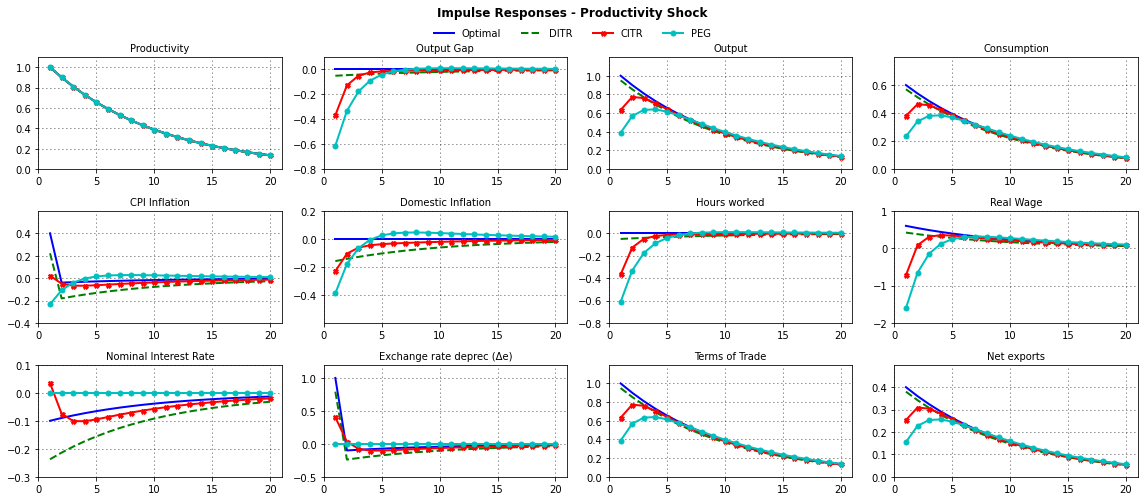
\includegraphics[width=1\textwidth]{img/Prod_shock_rep.png}
\end{figure}

A positive productivity shock lowers the marginal cost of firms. So, they would like to lower the prices to increase demand, but just a fraction of them is allowed to do so, because of price rigidity. To incentive demand, the Central Bank reacts immediately, cutting interest rates. As the economy is open, there's another demand channel: the exported goods. With more productivity, domestic prices become relatively lower, what improves the terms of trade. CPI inflation increases in the fist period because of imported goods, which are relatively more expensive. Net exports increase, as the rest of the world demands more domestic products as they are cheaper. Higher output (to match the potential) means firms have to hire more workers, which increases the demand for labour, increasing the real wages. Higher wages leads to higher consumption (also driven to lower real interest rates).

\vspace{6pt}

The dynamics of the Domestic Inflation Taylor Rule (DITR) is almost the same as the optimal policy. The difference is that the domestic inflation falls because of the productivity shock. The monetary authority then responds lowering the interest rates, but more than in the case of optimal policy\footnote{$r_t^{optimal} = \overline{rr}_t + \phi_{\pi}\pi_{H,t} = \rho + \sigma_\alpha \Gamma (1 - \rho_a) a_t + \alpha \sigma_\alpha (\Theta + \Psi)(\Et[y_{t+1}^*] - y_t^*) + \phi_{\pi}\pi_{H,t} = r_t^{DITR} + \sigma_\alpha \Gamma (1 - \rho_a) a_t + \alpha \sigma_\alpha (\Theta + \Psi)0 > r_t^{DITR}$, as $\sigma_\alpha>0$, $\Gamma>0$, $\rho_a<1$ and $a_t>0$}. It seems strange that a mores stimulative monetary policy leads to less demand and inflation. As all effects are instantaneous, with this policy the output gap is not closed. As prices are not flexible, a fraction of firms can't lower their prices, so the demand for their products decrease, which results in lower demand for workers (compared to the optimal policy) and less hours worked. With a weak demand, the domestic inflation falls which explains the lower nominal interest rate. The CPI increases (not too much) because of the improvement of the terms of trade (imported goods are more expensive due to exchange rate depreciation). It's interesting to note that the real exchange rate is less negative in the DITR compared to the optimal policy.   

\vspace{6pt}

Now comparing the CPI Inflation Taylor Rule (CITR) to the DITR, we can see that the output gap closes more slowly (recall that the openess of the economy was calibrated to 0.4), as the monetary authority doesn't cut the interest rates in the first period. As a result, as firms can't adjust their prices and without stimulative demand, the increase in output is just due to the higher productivity. A fraction of firms stay with higher prices, so they need to fire workers, what lowers the labour demand and decreases the real wage. A part of this negative effect is compensated by the higher external demand, but this effect isn't so strong because of less depreciation rate. As a result in the first period the output and consumption increase is less pronounced than the two policies described above. The hump-shape appears because if the expansionary monetary policy from the second period on. 

\vspace{6pt}

Finally, the PEG policy is the less effective one in this model. By hypothesis, there's no exchange rate depreciation and no interest rate change, as there were no changes on the external interest rates. The improvement in the terms of trade reflects only the price dynamics of the domestic economy, which is weaker than in the other three policies. Domestic inflation then falls sharply and this effect is so strong that the CPI falls too. Firms fire even more workers than in the CITR policy which means also lower real wages than all other policies. Consumption and output increase by less than in the case of CITR. In this case, the hump-shape is due to the deflation in the CPI, which results in a negative real interest rate. With the exception of the nominal interest rate, after the fifth period the trajectories of all other variables converge.

\subsection{World output shock}

This shock can be seen as a productivity shock in the rest of the world and the corresponding monetary policy optimal response. As $y_t^*=c_t^*$, there's a greater demand of goods imported from the small economy. As the shock now is not in the domestic economy (there's no domestic output gap to stabilize), the optimal monetary policy coincides with the DITR.

\begin{figure}[H]
\centering
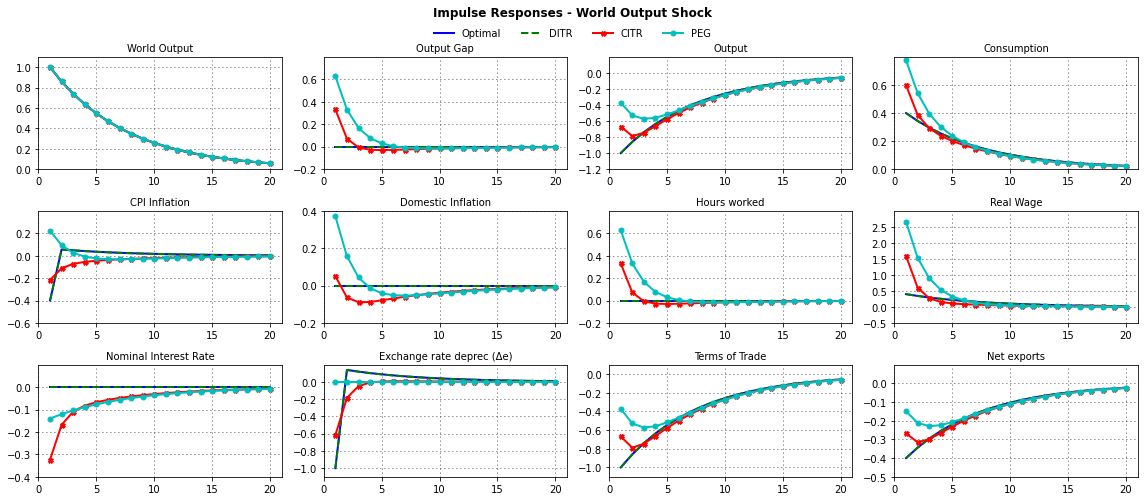
\includegraphics[width=1\textwidth]{img/y_star_shock_rep.png}
\end{figure}

A productivity shock in the rest of the world deteriorates the terms of trade of the domestic economy, as the imported goods are now relatively cheaper, what decreases the net exports (from an increase in imports and decrease in exports simultaneously). As there's no domestic inflation, the exchange rate appreciation reflects fully the deterioration of the terms of trade. The CPI inflation falls due to lower price of imported goods. The real wage increases due to the CPI deflation, which increases consumption. Even with higher consumption, lower output is the result of lower domestic demand (import goods are cheaper) and less exports (lower demand due to higher relative prices). 

For the CITR, as the Central Bank reacts to the whole CPI (which falls because of cheaper imported prices) reducing nominal interest rates which stimulates domestic demand above the potential (as the domestic productivity didn't change), opening the output gap. To work above potential, firms need to hire more workers, what increases the labour demand, resulting in higher wages. Higher wages and hours worked leads to higher domestic consumption, which prevents output to fall less than with the DITR. The output movement is directly reflected in the terms of trade. Due to less deterioration of the terms of trade, the nominal exchange rate doesn't appreciate too much, what helps a little the net exports.\\

Analysing the PEG policy, we can see that although it worsens less the terms of trade and, consequently, the net exports, the output gap is more positive, which means a lower fall of domestic output, resulting from higher domestic consumption resulting from higher real wages and even more hours worked compared with CITR. This impact is so strong that it increases the domestic inflation and also the CPI inflation. The nominal interest rate is the necessary to maintain a fixed exchange rate.

\section{Modification}
We include wage stickiness following \cite{erceg} and \citet[Chap.~6]{gali2015} in the small open economy model. This framework adds imperfect competition in the labor market and considers unions that can define labor supply and set nominal wages aiming to maximize workers' utility and that decision is subject to nominal rigidities following Calvo, with the same mechanism of the price setting by the firms. This modification changes the consumer problem (as they do not decides individually their work hours) and the firms' (by way of technology), while the external sector relations and the monetary policy rules are unaffected.

\subsection{Firms}
Each representative firm $j$ now uses a continuum of different labor types ($x \in [0,1]$) as inputs:

\begin{equation}
    Y_t(j) = A_t N_t(j) \quad N_t(j) \equiv \left( \int^1_0 N_t(j, \ell)^{\frac{\zeta-1}{\zeta}} d\ell \right)^{\frac{\zeta}{\zeta-1}}
\end{equation}

Where $\zeta$ represents the elasticity of substitution among labor varieties and $W_t(\ell)$ is the nominal wage per unit of $\ell$-type labor. Analogously to the consumer problem that solve for the optimal demand for each type of good given the individual aggregate consumption, for the firm cost minimization problem given $N_t(j)$ we have that the optimal demand for $n$-type labor is:

\begin{equation}
    N_t(j,\ell) = \left(\frac{W_t(\ell)}{W_t} \right)^\zeta N_t(j) \quad \textrm{ where } \ W_t \equiv \left(\int^1_0 W_t(\ell)^{1-\zeta} d\ell \right)^{\frac{1}{1-\zeta}}
\end{equation}

The $W_t$ and $N_t(j)$ above are such that in aggregate terms $\int^1_0 W_t(\ell) N_t(j,\ell) d\ell = W_t N_t(j)$. It follows that the firms' price setting problem remains unchanged as marginal cost is constant due to constant returns to scale and $W_t$ is calculated by the aggregator above.

\subsection{Households}
Moreover we assume that all consumers homogeneously supply all the labor types implying that his income is given by $\int^1_0 W_t(\ell) N_t(\ell) d\ell$, leading to the same problem discussed in the original model:

\begin{equation}
    \max_{C_t} E_0 \sum^\infty_{t=0} \beta^t \left[\frac{C_t^{1-\sigma}}{1-\sigma} - \frac{N_t^{\varphi+1}}{\varphi+1} \right] \hspace{1em}  \textrm{ st. } \hspace{1em} \forall t, \hspace{0.8em} P_t C_t + \Et[Q_{t,t+1} D_{t+1}] \leq D_t +  \int^1_0 W_t(\ell) N_t(\ell) d\ell + T_t
\end{equation}

The major difference is that now the consumers do not chose anymore the hours worked, thus labor income is now exogenous and the maximization problem solution consists only in the Euler equation showed in (\ref{euler}). The endogenous labor doesn't affect the consumption decision because the preferences are separable.

\subsection{Wage setting}

The model assumes that there exists a continuum of representative unions that can determine the nominal wages for each labor type. Analogously to the price setting problem we assume that each union is not completely free to adjust the wage at any period, but only a random selected fraction of them with measure $\varsigma$ can reset the wages in a given period, while the remaining fraction must keep the nominal wage unchanged. The union wage setting problem considers the utility maximization of the workers, taking as exogenous the other union decisions and the labor demand by the firms. Formally:

\begin{equation}
    \label{wage_setting}
    \max_{W_t^*} \Et \sum^\infty_{k=0} (\beta \varsigma)^k \left( \frac{C_{t+k}^{-\sigma}}{C_t^{-\sigma}} \frac{P_t}{P_{t+k}} W_t^* N_{t+k|t} - \frac{N_{t+k|t}^{1+\varphi}}{1+\varphi} \right)Z_{t+k} \quad \textrm{such that} \quad N_{t+k|k} = \left(\frac{W_t^*}{W_{t+k}} \right)^{-\zeta} \left(\int_0^1 N_t(j) dj \right)
\end{equation}

\begin{minipage}{0.3\textwidth}
    The first order condition is given by:
\end{minipage} 
\begin{minipage}{0.69\textwidth}
    \begin{equation}
        \label{foc_wage}
        \sum^\infty_{k=0} (\beta \varsigma)^k \Et \left[N_{t+k|t} Z_{t+k} \left(\frac{C_{t+k}^{-\sigma} W_t^*}{P_{t+k}} - \Xi N_{t+k|t}^\varphi \right) \right] = 0
    \end{equation}
\end{minipage} 

where $\Xi = \frac{\zeta}{\zeta-1}$. Log-linearizing and rearranging the expression above and defining $\xi = \ln(\Xi)$ we get:

\begin{equation}
    w_t^* = (1 - \beta \varsigma) \sum^\infty_{k=0} (\beta \rho)^k \Et[\xi +  \sigma c_{t+k} + \varphi n_{t+k|t} + p_{t+k}]
\end{equation}


Log-linearizing the constraint in (\ref{wage_setting}) we obtain that $n_{t+k|t} = -\zeta w_t^* + \zeta w_{t+k} + n_{t+k}$, thus:

\begin{equation}
    w_t^* = (1 - \beta \varsigma) \sum^\infty_{k=0} (\beta \rho)^k \Et[\xi +  \sigma c_{t+k} + \varphi( \zeta w_{t+k} -\zeta w_t^* + n_{t+k}) + p_{t+k}]
\end{equation}

\begin{equation}
    w_t^* = \frac{1-\beta \varsigma}{1 + \zeta \varphi} \sum^{\infty}_{k=0} (\beta \varsigma)^k \Et[\xi + \sigma c_{t+k} + \varphi n_{t+k} + \zeta \varphi w_{t+k} + p_{t+k}]
\end{equation}

\begin{minipage}{0.3\textwidth}
    Writing in a recursive form:
\end{minipage} 
\begin{minipage}{0.69\textwidth}
    \begin{equation}
        \label{opt_wage}
        w_t^* = \beta \varsigma \Et[w^*_{t+1}] + (1 - \beta \varsigma) \left[w_t - (1+\zeta \varphi)^{-1} (w_t^R  - \sigma c_t - \varphi n_t - \xi) \right]
    \end{equation}
\end{minipage} 

\subsection{Wage inflation dynamics}
The wage inflation is defined as $\Pi_{w,t} = \frac{W_t}{W_{t-1}}$ or, log-linearizing, $\pi_{w,t} = w_t - w_{t-1}$. As we defined real wage $W_t^R = \frac{W_t}{P_t}$ we can derive a relation between goods and wage inflation:

\vspace{6pt}

\begin{minipage}{0.5\textwidth}
    \begin{equation}
        \Pi_{w,t} = \frac{W_t}{W_{t-1}} = \frac{W_t^R P_t}{W_{t-1}^R P_{t-1}} = \frac{W_t^R}{W_{t-1}^R}\Pi_t
    \end{equation}
\end{minipage} 
\begin{minipage}{0.49\textwidth}
    \begin{equation}
        \label{wage_inflation}
        \textrm{Log-linearizing:} \ \ \ \pi_{w,t} = w_t^R - w_{t-1}^R + \pi_t
    \end{equation}
\end{minipage} 

\begin{minipage}{0.5\textwidth}
    The aggregate wage dynamics is given by:
\end{minipage} 
\begin{minipage}{0.49\textwidth}
    \begin{equation}
        W_t = \left(\varsigma W_{t-1}^{1-\zeta} + (1-\varsigma) (W_t^*)^{1-\zeta} \right)^{\frac{1}{1-\zeta}}
    \end{equation}
\end{minipage} 

\vspace{6pt}

\begin{minipage}{0.4\textwidth}
    Log-linearizing and calculating $\pi_{w,t}$:
\end{minipage} 
\begin{minipage}{0.59\textwidth}
    \begin{equation}
        w_t = \varsigma w_{t-1} + (1-\varsigma) w_t^* \Rightarrow \pi_{w,t} = (1-\varsigma)(w_t^* - w_{t-1})
    \end{equation}
\end{minipage} 

\vspace{6pt}

Substituting the expression for $w_t^*$ found in (\ref{opt_wage}) and rearranging:

\begin{equation}
    \label{wage_pc}
    \pi_{w,t} = \beta \Et[\pi_{w,t+1}] - \Lambda (w_t^R  - \sigma c_t - \varphi n_t - \xi)
\end{equation}

where $\Lambda \equiv \frac{(1-\varsigma)(1- \beta \varsigma)}{\varsigma(1+ \zeta \varphi)}$.

\subsection{Equilibrium}
The new log-linearized equilibrium is the same showed in (\ref{sistema_loglin}) but removing the labor supply equation (\ref{labour_supply_log}) and adding (\ref{wage_pc}) and (\ref{wage_inflation}). Note that this new model generalizes the original one in \cite{gali_monacelli}: assuming that workers have no market power to set wages due to perfect substitutability among labor types, that is $\zeta \to \infty$ (thus $\Xi \to 1$ and $\xi \to 0$), and there is not wage stickiness, $\varsigma \to 0$ (thus $\Lambda \to \infty$) we are back to the baseline model. The order of variables in the code is then:

\begin{table}[H]
    \centering
    \begin{tabular}{ccccccccccccccccc}
        \hline
        $x_t$ & $y_t^*$ & $\pi_{H,t}$ & $a_t$ & $r_t$ & $\overline{y}_t$ & $y_t$ & $c_t^*$ & $s_t$ & $q_t$ & $c_t$ & $\pi_t$ & $\Delta e_t$ & $\overline{mc}_t$ & $n_t$ & $w_t^R$ & $\pi_{w,t}$\\
        0 & 1 & 2 & 3 & 4 & 5 & 6 & 7 & 8 & 9 & 10 & 11 & 12 & 13 & 14 & 15 & 16 \\
        \hline
    \end{tabular}
\end{table}

\section{New implications for the static and dynamics properties of the model}

\subsection{Steady state}
Using the first order condition in the wage setting problem in (\ref{foc_wage}) evaluated in the steady state the wage supply becomes $W^R = \Xi N^\varphi C^\sigma$. Thus, the exact same steady state found in (\ref{ser}) must hold. The only change is the substitution of the labor supply equation (\ref{ser}a) to the expression above:

\begin{subequations}
    \label{ser_wage}
    \begin{minipage}{0.39\textwidth}
        \begin{align}
            & \Xi C^\sigma N^\varphi = W^R \\
            &\mathcal{Q} = \left[(1-\alpha)S^{\eta-1} + \alpha \right]^{\frac{1}{\eta-1}}\\
            &Y =  N
        \end{align}
    \end{minipage}
    \begin{minipage}{0.6\textwidth}
        \begin{align}
            &1 = W^R \left[(1-\alpha) + \alpha S^{1-\eta} \right]^{\frac{1}{1-\eta}} (1 - \tau) \mathcal M\\
            &C = \mathcal Q^{\frac{1}{\sigma}}\\
            &Y = C \left[(1-\alpha) + \alpha S^{1-\eta} \right]^{\frac{\eta}{1-\eta}} \left[(1-\alpha)  +  \alpha \mathcal S^{\gamma - \eta} \mathcal Q^{\eta - \frac{1}{\sigma}} \right]
        \end{align}
    \end{minipage}
\end{subequations}

\vspace{6pt}

It is immediate that if $\zeta \to \infty$ then $\Xi \to 1$ and the system above results in the same of the original model. Assuming the same calibration showed in section 4 and, for the new parameters, adopting $\varsigma = 0.75$ (consistent with 1 year as average time to change wages) and $\zeta = 4$ (following \cite{erceg}, that considered a wage markup of $1/3$) we obtain that the steady state values are identical to the original model except the real wage:

\begin{table}[H]
    \centering
    \begin{tabular}{clcc}
        \hline
        \multirow{2}*{\textbf{Variable}} & \multirow{2}*{\textbf{Description}} & \textbf{Original} & \textbf{Model with}\\
        & & \textbf{Model} & \textbf{Price Stickiness} \\
        \hline
        $Y$ & Output & 1.13622 & 1.13622 \\
        $C$ & Consumption & 1.07964 & 1.07964 \\
        $W^R$ & Real wage & 1.58367 & 2.11156 \\
        $C/Y$ & Consumption-to-GDP Ratio & 0.95020 & 0.95020 \\
        $S$ & Terms of trade & 1.13622 & 1.13622 \\
        $NX/Y$ & New exports in terms of domestic output & $0.00000$ & $0.00000$\\
        $(R^4 -1)$ & Real annual interest rate &  0.04102 &  0.04102\\
        \hline
    \end{tabular}
\end{table}

\subsection{Dynamic Properties}

\begin{minipage}{0.67\textwidth}
    Again, simulating 1000 samples with 201 periods, we obtained the following dynamic properties. The previously obtained optimal policy rule $r_t = \overline{rr}_t + \phi_\pi \pi_{H,t}$ is no longer optimal in that new framework due to change in the welfare cost. We proceed our comparison with only DITR, CITR and Peg.
    \begin{table}[H]
        \centering
        \begin{tabular}{lcccccc}
            \hline
            & \multicolumn{2}{c}{DI Taylor} & \multicolumn{2}{c}{CPI Taylor} & \multicolumn{2}{c}{Peg}\\
            & Model & Modif.  & Model & Modif.  & Model & Modif. \\
            &  sd\% & sd\% & sd\% & sd\% & sd\% & sd\% \\
            \hline
            Output &  0.66 & 1.81 & 0.70 & 1.75 & 0.84 & 1.43 \\
            Domestic inflation & 0.27 & 0.37 & 0.26 & 0.33 & 0.35 & 0.25 \\
            CPI inflation & 0.40 & 0.41 & 0.26 & 0.33 & 0.21 & 0.15 \\
            Nominal int. rate & 0.40 & 0.55 & 0.40 & 0.50 & 0.21 & 0.20 \\
            Terms of trade & 1.43 & 1.29 & 1.33 & 1.12 & 1.08 & 1.03 \\
            Nominal depr. rate & 0.85 & 0.61 & 0.52 & 0.43 & 0.00 & 0.00 \\
            \hline
            \multicolumn{5}{l}{\textit{Note: } Sd denotes standard deviation in \%}
        \end{tabular}
    \end{table}
\end{minipage}
\begin{minipage}{0.02\textwidth}
\end{minipage}
\begin{minipage}{0.30\textwidth}
    What we can see here comparing these two models is that in this case the output is much more volatile, more than twice than the standard model, in the case DITR and CITR but not the volatility doesn't fall too much with the peg policy.The domestic inflation turns to be more volatile with both Taylor rule specifications, but is less volatile when the peg is chosen. The terms of trade are less favorable with all three policies and the nominal depreciation rate is lower for both Taylor rule policies, compared to the baseline.
\end{minipage}


\subsection{Impulse Response Functions}
The new calculated impulse response functions to both shocks are:

\begin{figure}[H]
\centering
\includesvg[inkscapelatex=false, width=0.9\textwidth]{img/figure3.svg}
\end{figure}

\begin{figure}[H]
\centering
\includesvg[inkscapelatex=false, width=0.9\textwidth]{img/figure4.svg}
\end{figure}

Explicar! Ressaltar que as variáveis reais / quantidades reagem mais fortemente dada a maior rigidez nominal\\

\begin{figure}[H]
\centering
\includesvg[inkscapelatex=false, width=0.9\textwidth]{img/figure5.svg}
\end{figure}

\subsubsection{Welfare Losses}
Following the derivation for welfare losses in a closed economy with wage stickiness in \citet[Appendix.~6.1]{gali2015} and in a open economy with openness index $\alpha$ in \cite{rhee} the the expected welfare losses as fraction of steady state consumption are given by:

\begin{equation}
    \mathbb V = -\frac{(1-\alpha)}{2} \left[ (1 + \varphi) var(x_t) + \frac{\varepsilon}{\lambda} var(\pi_t) + \frac{\zeta}{\Lambda} var(\pi_{w,t}) \right] 
\end{equation}

Now calculating the contributions to welfare losses in the new model, considering different levels of wage rigidities:

\begin{table}[H]
    \centering
    \begin{tabular}{lcccc}
        \hline
        &  DI Taylor & CPI Taylor & Peg\\
        \hline
        \multicolumn{4}{c}{No wage rigidity: $\varsigma = 0$}\\
        Var(Domestic infl.) & 0.01506 & 0.01570 & 0.04082\\
        Var(Output gap) & 0.00088 & 0.00224 & 0.00662\\
        Var(Wage infl.) & 0.00000 & 0.00000 & 0.00000\\
        Total & 0.01594 & 0.01794 & 0.04744\\
        \multicolumn{4}{c}{Low wage rigidity: $\varsigma = 0.25$}\\
        Var(Domestic infl.) & 0.01587 & 0.01334 & 0.02549\\
        Var(Output gap) & 0.00106 & 0.00420 & 0.01076\\
        Var(Wage infl.) & 0.01473 & 0.02009 & 0.02418\\
        Total & 0.03167 & 0.03763 & 0.06043\\
        \multicolumn{4}{c}{Intermediate wage rigidity: $\varsigma = 0.50$}\\
        Var(Domestic infl.) & 0.02171 & 0.01706 & 0.01889\\
        Var(Output gap) & 0.00353 & 0.00764 & 0.01460\\
        Var(Wage infl.) & 0.05409 & 0.04948 & 0.01989\\
        Total & 0.07933 & 0.07417 & 0.05338\\
        \multicolumn{4}{c}{Standard wage rigidity: $\varsigma = 0.75$}\\
        Var(Domestic infl.) & 0.03002 & 0.02320 & 0.01485\\
        Var(Output gap) & 0.02904 & 0.02963 & 0.02146\\
        Var(Wage infl.) & 0.29458 & 0.21234 & 0.01422\\
        Total & 0.35364 & 0.26516 & 0.05053\\
        \hline
        \multicolumn{4}{l}{\textit{Note: } Values are \% units of steady state consumption}
    \end{tabular}
\end{table}

Comentar! Quanto mais rígido comparativamente a PEG fica superior

\section{Conclusion}
a


\appendix
\section{Consumer problem}
The consumer problem is 
\begin{equation}
    \displaystyle \max_{C_t,N_t} \ E_0 \sum_{t=0}^\infty \beta^tU(C_t,N_t) = \max_{C_{H,t},C_{F,t},N_t} \ E_0 \sum_{t=0}^\infty \beta^t U \left(\left[ (1-\alpha)^{\frac{1}{\eta}} (C_{H,t})^{\frac{\eta-1}{\eta}} + \alpha^{\frac{1}{\eta}} (C_{F,t})^{\frac{\eta-1}{\eta}} \right]^{\frac{\eta}{\eta-1}},N_t \right)
\end{equation}

Substituting the equations (\ref{index_eqs}) with the definition of the indices, and using the consumer's restriction with equality, we can write the Lagrangean below:

\begin{equation*}
    \mathcal{L} = \displaystyle E_t \sum_{t=0}^\infty \beta^t U \left(\left[ (1-\alpha)^{\frac{1}{\eta}} \left [\displaystyle \left( \int_0^1 C_{H,t}(j)^{\frac{\varepsilon-1}{\varepsilon}}dj \right) ^{\frac{\varepsilon}{\varepsilon-1}} \right]^{\frac{\eta-1}{\eta}} + \alpha^{\frac{1}{\eta}} \left[ \displaystyle \left( \int_0^1 \left( \displaystyle \left( \int_0^1 C_{i,t}(j)^{\frac{\varepsilon-1}{\varepsilon}}dj \right) ^{\frac{\varepsilon}{\varepsilon-1}} \right)^{\frac{\gamma-1}{\gamma}}di \right) ^{\frac{\gamma}{\gamma-1}} \right]^{\frac{\eta-1}{\eta}} \right]^{\frac{\eta}{\eta-1}},N_t \right)
\end{equation*}
\begin{equation}
    + \Upsilon_t \left(D_t + W_tN_t + Tt \displaystyle - \int_0^1 P_{H,t}(j)C_{H,t}(j)dj - \int_0^1\int_0^1 P_{i,t}(j)C_{i,t}(j)dj\ di - E_t\{ Q_{t,t+1}D_{t+1}\}\right)
\end{equation}

Now we can calculate the MRS (marginal rate of substitution) between $C_{H,t}(j)$ and $C_{H,t}$, as by the optimal allocation (and well behaved utility functions), it has to be the rate of prices in every period of time (otherwise the consumer could by a little less of the product with relative higher price and buy another with relative lower price, increasing his utility).

\begin{equation}
    \displaystyle \frac{\displaystyle \frac{\partial U(C_t,N_t)}{\displaystyle \partial C_{H,t}(j)}}{\frac{\displaystyle \partial U(C_t,N_t)}{\displaystyle \partial C_{H,t}}} = \frac{\displaystyle U_c(C_t,N_t) \left( (1-\alpha) \frac{C_t}{C_{H,t}} \right)^{\frac{1}{\eta}} \int_0^1 \left(\frac{C_{H,t}}{C_{H,t}(j)}\right)^{\frac{1}{\varepsilon}}dj}{\displaystyle U_c(C_t,N_t) \left( (1-\alpha) \frac{C_t}{C_{H,t}} \right)^{\frac{1}{\eta}}} = \frac{\displaystyle \int_0^1P_{H,t}(j)dj}{P_{H,t}}
\end{equation}

After simplifying, we get the (\ref{Chj_demand}) equation.

\begin{equation}
    \displaystyle \int_0^1 \left(\frac{C_{H,t}}{C_{H,t}(j)}\right)^{\frac{1}{\varepsilon}}dj = \displaystyle \int_0^1 \frac{P_{H,t}(j)}{P_{H,t}}dj  \ \ \Rightarrow \ \ C_{H,t}(j)= \left( \frac{P_{H,t}(j)}{P_{H,t}} \right)^{-\varepsilon}C_{H,t}
\end{equation}
    
Similarly, with the MRS calculation we arrive at (\ref{Cij_demand}) and (\ref{Ci_demand}).

\begin{equation}
    \displaystyle \frac{\displaystyle \frac{\partial U(C_t,N_t)}{\displaystyle \partial C_{i,t}(j)}}{\frac{\displaystyle \partial U(C_t,N_t)}{\displaystyle \partial C_{i,t}}} = \frac{\displaystyle U_c(C_t,N_t) \left( \alpha \frac{C_t}{C_{F,t}} \right)^{\frac{1}{\eta}} \int_0^1 \left(\frac{C_{F,t}}{C_{i,t}}\right)^{\frac{1}{\gamma}} \int_0^1 \left(\frac{C_{i,t}}{C_{i,t}(j)}\right)^{\frac{1}{\varepsilon}}dj \ di }{\displaystyle U_c(C_t,N_t) \left( \alpha \frac{C_t}{C_{F,t}} \right)^{\frac{1}{\eta}} \int_0^1 \left(\frac{C_{F,t}}{C_{i,t}}\right)^{\frac{1}{\gamma}} di} = \frac{\displaystyle \int_0^1P_{i,t}(j)dj}{P_{i,t}}
\end{equation}

\begin{equation}
    \displaystyle \int_0^1 \int_0^1 \left(\frac{C_{F,t}}{C_{i,t}}\right)^{\frac{1}{\gamma}} \left(\frac{C_{i,t}}{C_{i,t}(j)}\right)^{\frac{1}{\varepsilon}}dj \ di = \int_0^1 \int_0^1 \frac{\displaystyle P_{i,t}(j)}{P_{i,t}} \left(\frac{C_{F,t}}{C_{i,t}}\right)^{\frac{1}{\gamma}} dj \ di \ \ \Rightarrow \ \
     C_{i,t}(j) = \left( \frac{\displaystyle P_{i,t}(j)}{P_{i,t}} \right)^{-\varepsilon}C_{i,t} 
\end{equation}

\begin{equation}
    \displaystyle \frac{\displaystyle \frac{\partial U(C_t,N_t)}{\displaystyle \partial C_{i,t}}}{\frac{\displaystyle \partial U(C_t,N_t)}{\displaystyle \partial C_{F,t}}} = \frac{\displaystyle U_c(C_t,N_t) \left( \alpha \frac{C_t}{C_{F,t}} \right)^{\frac{1}{\eta}} \int_0^1 \left(\frac{C_{F,t}}{C_{i,t}}\right)^{\frac{1}{\gamma}} di }{\displaystyle U_c(C_t,N_t) \left( \alpha \frac{C_t}{C_{F,t}} \right)^{\frac{1}{\eta}} } = \frac{\displaystyle \int_0^1P_{i,t}di}{P_{F,t}} \ \ \Rightarrow \ \ \left(\frac{C_{F,t}}{C_{i,t}}\right)^{\frac{1}{\gamma}} = \frac{P_{i,t}}{P_{F,t}}  \ \ \Rightarrow \ \ C_{i,t} = \left( \frac{P_{i,t}}{P_{F,t}} \right)^{-\gamma}C_{F,t}
\end{equation}

We can also calculate the optimal share of imported goods.

\begin{equation}
    \displaystyle \frac{\displaystyle \frac{\partial U(C_t,N_t)}{\displaystyle \partial C_{F,t}}}{\frac{\displaystyle \partial U(C_t,N_t)}{\displaystyle \partial C_t}} = \frac{\displaystyle U_c(C_t,N_t) \left( \alpha \frac{C_t}{C_{F,t}} \right)^{\frac{1}{\eta}}}{\displaystyle U_c(C_t,N_t) } = \frac{P_{F,t}}{P_t} \ \ \Rightarrow \ \ \alpha \frac{C_t}{C_{F,t}} = \left( \frac{P_{F,t}}{P_t} \right)^\eta \ \ \Rightarrow \ \ C_{F,t} = \alpha \left( \frac{P_{F,t}}{P_t} \right)^{-\eta}C_t;
\end{equation}

\begin{equation}
    C_{H,t} = (1-\alpha)\left( \frac{P_{H,t}}{P_t} \right)^{-\eta}C_t
\end{equation}

It remains to do the aggregation of the budget constraint of the representative consumer:

\begin{equation}
    \displaystyle \int_0^1 P_{H,t}(j)C_{H,t}(j)dj = \int_0^1P_{H,t}(j)\left( \frac{P_{H,t}(j)}{P_{H,t}}\right)^{-\varepsilon}C_{H,t}dj = \frac{C_{H,t}}{P_{H,t}^{-\varepsilon}}\int_0^1P_{H,t}(j)^{1-\varepsilon}dj = \frac{C_{H,t}}{P_{H,t}^{-\varepsilon}}P_{H,t}^{1-\varepsilon} = P_{H,t}C_{H,t}
\end{equation}

Doing twice the same steps as above (using the demand functions and price indices), we can aggregate the consumer's expenditure on imported goods. As the total expenditure in goods is the sum of domestic goods and imported goods, we achieve the consumer's problem described in (\ref{cons_problem}).

\begin{equation}
    \displaystyle \int_0^1\int_0^1 P_{i,t}(j)C_{i,t}(j)dj\ di = \int_0^1\int_0^1 P_{H,t}(j)\left( \frac{P_{i,t}(j)}{P_{i,t}}\right)^{-\varepsilon}C_{i,t}dj \ di = \int_0^1 P_{i,t}C_{i,t} di = P_{F,t}C_{F,t}  
\end{equation}

\section{Labor subsidy definition}
As the model depends on imperfect competition assumption, the firms have market power implying that competitive equilibrium is not Pareto Optimal due to lower production and hiring. In this case, the domestic benevolent social planner maximizes the representative household discounted utility subject to technology (\ref{technology}), domestic/foreign consumption relation due to international risk sharing (\ref{consumption}) and market clearing (\ref{output_st}). For a analytically tractable solution we need to impose $\gamma = \sigma = \eta = 1$ (as adopted in the calibration). The problem becomes:

$$\max_{C_t, N_t} E_0 \sum^\infty_{t=0} \beta^t \left[\ln(C_t) - \frac{N_t^{\varphi+1}}{\varphi+1} \right] \ \textrm{ s.t. } \begin{matrix}
    Y_t = A_t N_t\\
    C_t = C_t^* \mathcal Q_{t}\\
    Y_t = C_t S_t^\alpha
\end{matrix}$$

By (\ref{real_rate}) with $\gamma = \sigma = \eta = 1$ we have that $\mathcal{Q}_t = S_t^{1-\alpha}$, and using the global market clearing condition in (\ref{world_equilibrium}): $Y_t^* = C_t^*$ we rewrite the social planner problem:

$$\max_{C_t, N_t} E_0 \sum^\infty_{t=0} \beta^t \left[\ln(C_t) - \frac{N_t^{\varphi+1}}{\varphi+1} \right] \ \textrm{ s.t. } \begin{matrix}
    C_t = (A_t N_t)^{1-\alpha}(Y_t^*)^\alpha
\end{matrix}$$

As this problem is a static one we can solve separately for $C_t$ and $N_t$ at any period. The Lagrangean and the first order conditions are:

\begin{equation*}
    \begin{split}
        \mathcal L = & \ln(C_t) - \frac{N_t^{\varphi+1}}{\varphi+1} - \lambda_t(C_t - (A_t N_t)^{1-\alpha}(Y_t^*)^\alpha) \\
        (C_t) \ & \frac{1}{C_t} - \lambda_t = 0\\
        (N_t) \ & -N_t^\varphi + \lambda_t (Y_t^*)^\alpha (1 - \alpha) A_t^{(1 - \alpha)}N_t^{-\alpha} = 0\\
    \end{split}
\end{equation*}

Manipulating we get that $N_t^{1+\varphi} = N^{1+\varphi} = (1-\alpha)$. In the competitive steady state in (\ref{ser}) again assuming $\gamma = \sigma = \eta = 1$ we obtain that $\frac{1}{\mathcal M} = (1-\tau) N^{1+\varphi}$. So, if the subsidy is such that $(1-\tau) = \frac{1}{(1-\alpha) \mathcal M}$ the steady state employment level coincides to Pareto optimal and, then, the efficiency is restored. Note that the solution above holds only for this specific parameter selection.

\section{Optimal price setting}
The firms optimal price setting problem following the Calvo's model is given by:

\begin{equation}
    \overline{P}_{H,t} = \max_{\overline{P}_{H,t}} \sum^\infty_{k=0} \theta^k \Et \left[ Q_{t, t+k}[Y_{t+k}(j) (\overline {P}_{H,t} - MC_{t+k} P_{H,t+k})] \right]
\end{equation}

The domestic demand for a specific variety is $C_{H,t}(j) = \left( \frac{P_{H,t}(j)}{P_{H,t}} \right)^{-\varepsilon} C_{H, t}$ if the price remains unchanged at $\overline {P}_{H,t}$ until $t+k$ period then: $C_{t+k}(j) = \left( \frac{\overline {P}_{H,t}(j)}{P_{H,t+k}}\right)^{-\varepsilon} C_{H, t+k}$. Similarly the foreign consumption of this domestic good is $C^i_{t+k}(j) = \int^1_0 \left( \frac{\overline {P}_{H,t}(j)}{P_{H,t+k}} \right)^{-\varepsilon} C^i_{H, t+k} di$. Market clearing imposes that:

\begin{equation}
    Y_{t+k}(j) = C_{H,t+k}(j) + \int_0^1 C^i_{H, t+k}(j) di = \left( \frac{\overline{p}_{H,t}}{P_{H,t+k}} \right)^{-\varepsilon} \left(C_{H,t+k} +  \int_0^1 C^i_{H, t+k} di \right) \equiv \left( \frac{\overline{p}_{H,t}}{P_{H,t+k}} \right)^{-\varepsilon} \tilde C_{H,t+k}
\end{equation}

Substituting $Q_{t, t+k}$ for the expression obtained in the consumer problem and $Y_{t+k}(j)$ for the expression above in the firms problem:

\begin{equation}
    \overline{p}_{H,t} = \max_{\overline{p}_{H,t}} \sum^\infty_{k=0} \theta^k \Et \left[ \beta^k \left( \frac{C_{t+k}}{C_t} \right)^{-\sigma} \left( \frac{P_{t}}{P_{t+k}} \right) \left( \frac{\overline{p}_{H,t}}{P_{H,t+k}} \right)^{-\varepsilon} \tilde C_{H,t+k} (\overline{p}_{H,t} - MC_{t+k} P_{H,t+k})  \right]
\end{equation}

Calculating the first order condition with respect to $\overline{p}_{H,t}$ and rearranging we get:

\begin{equation}
    \overline{p}_{H,t} =  \frac{\Et\left[ \sum^\infty_{k=0} (\beta\theta)^k C_{t+k}^{-\sigma} \frac{1}{P_{t+k}}\tilde C_{H,t+k} P_{H,t+k} MC_{t+k} \mathcal M \right] }{\Et\left[ \sum^\infty_{k=0} (\beta\theta)^k C_{t+k}^{-\sigma} \frac{1}{P_{t+k}} \tilde C_{H,t+k}  \right]}
\end{equation}

In the zero inflation steady state $\overline{p}_{H,t} = P_{H,t} = P_{t} = P_H$, implying that, by the previous formula, $MC_{t}  = \frac{1}{\mathcal M} \equiv \frac{\varepsilon-1}{\varepsilon}$. Thus we define $\widehat{MC}_t = \frac{MC_t}{1/ \mathcal M}$ as the marginal cost deviation from steady state. Now using the price dynamics:

\begin{equation}
    P_{H,t} = [ \theta P_{H,t-1}^{1-\varepsilon} + (1-\theta) \overline{p}_{H,t}^{1-\varepsilon}]^\frac{1}{1-\varepsilon} \Rightarrow \Pi_{H,t} = \frac{P_{H,t}}{P_{H,t-1}} =  \frac{\left[ \theta P_{H,t}^{1-\varepsilon} + (1-\theta) \overline{p}_{H,t}^{1-\varepsilon}\right]^\frac{1}{1-\varepsilon}}{P_{H,t-1}} 
\end{equation}

\begin{equation}
    P_{H,t} = [ \theta P_{H,t-1}^{1-\varepsilon} + (1-\theta) \overline{p}_{H,t}^{1-\varepsilon}]^\frac{1}{1-\varepsilon} \Rightarrow \Pi_{H,t} = \frac{P_{H,t}}{P_{H,t-1}} =  \left[ \theta + (1-\theta) \frac{\overline{p}_{H,t}^{1-\varepsilon}}{P_{H,t-1}^{1-\varepsilon}} \right]^\frac{1}{1-\varepsilon} 
\end{equation}

Substituing $\overline{p}_{H,t}$ we reach:

\begin{equation}
    \Pi_{H,t} = \left[ \theta + \frac{(1-\theta)}{P_{H,t-1}^{1-\varepsilon}} \left(\frac{\Et\left[ \sum^\infty_{k=0} (\beta\theta)^k C_{t+k}^{-\sigma} \frac{1}{P_{t+k}}\tilde C_{H,t+k} P_{H,t+k} \widehat{MC}_{t+k}\right] }{\Et\left[ \sum^\infty_{k=0} (\beta\theta)^k C_{t+k}^{-\sigma} \frac{1}{P_{t+k}} \tilde C_{H,t+k}  \right]} \right)^{1-\varepsilon}\right]^\frac{1}{1-\varepsilon}
\end{equation}


Log-linearizing we get:

\begin{equation}
    \frac{\pi_{H,t} + p_{H,t-1}}{(1-\theta)(1-\beta \theta) } = \sum^\infty_{k=0} (\beta \theta)^k \Et[\widehat{mc}_{t+k} + p_{t+k}] 
\end{equation}

To obtain a recursive form, subtract for the same expression in $t+1$ multiplied by $\beta$, apply the Law of Iterated Expectations and rearrange:

\begin{equation}
    \frac{\pi_{H,t} - \beta \Et[\pi_{H,t+1}]}{(1-\theta)(1-\beta \theta) } = \sum^\infty_{k=0} (\beta \theta)^k \Et[\widehat{mc}_t + p_{t+k}]  - \beta \Et \sum^\infty_{k=0} (\beta \theta)^k  \mathbb E[\widehat{mc}_{t+1+k} + p_{t+k+1}] 
\end{equation}


\begin{equation}
    \pi_{H,t} = \beta \Et[\pi_{H,t+1}] + \lambda \widehat{mc}_t
\end{equation}

Where $\lambda \equiv \frac{(1-\theta) (1 - \beta \theta)}{\theta}$.

\section{Goods market clearing}
Market clearing in goods market imposes that, for each domestic good, the total production is equal to domestic + external demands:

\begin{equation}
    Y_{t}(j) = \left( \frac{P_{H,t}(j)}{P_{H,t}} \right)^{-\varepsilon} C_{H,t} + \left( \frac{P_{H,t}(j)}{P_{H,t}} \right)^{-\varepsilon} \int_0^1 C^i_{H, t} di
\end{equation}

Substituting $C_{H,t} = (1-\alpha) \left( \frac{P_{H,t}}{P_t} \right)^{-\eta} C_t$ and $C^i_{H,t} = \alpha \left( \frac{P_{H,t}}{\mathcal{E}_{i,t} P^i_{F,t}} \right)^{-\gamma} \left( \frac{P^i_{F,t}}{P^i_{t}} \right)^{-\eta} C^i_t$

\begin{equation}
    Y_{t}(j) = \left( \frac{P_{H,t}(j)}{P_{H,t}} \right)^{-\varepsilon} \left((1-\alpha) \left( \frac{P_{H,t}}{P_t} \right)^{-\eta} C_t +  \alpha \int_0^1 \left( \frac{P_{H,t}}{\mathcal{E}_{i,t} P^i_{F,t}} \right)^{-\gamma} \left( \frac{P^i_{F,t}}{P^i_{t}} \right)^{-\eta} C^i_t di \right)
\end{equation}

As $Y_t = \left[\int^1_0 Y_t(j)^{\frac{\varepsilon-1}{\varepsilon}} \right]^\frac{\varepsilon}{\varepsilon-1}$

\begin{equation}
    \label{}
    \begin{split}
    Y_{t} &= \left\{ \int^1_0 \left[ \left( \frac{P_{H,t}(j)}{P_{H,t}} \right)^{-\varepsilon} \left((1-\alpha) \left( \frac{P_{H,t}}{P_t} \right)^{-\eta} C_t +  \alpha \int_0^1 \left( \frac{P_{H,t}}{\mathcal{E}_{i,t} P^i_{F,t}} \right)^{-\gamma} \left( \frac{P^i_{F,t}}{P^i_{t}} \right)^{-\eta} C^i_t di \right)\right]^{\frac{\varepsilon-1}{\varepsilon}}dj \right\}^\frac{\varepsilon}{\varepsilon-1}\\
    Y_{t} &= \left\{ \int^1_0 \left( P_{H,t}(j)^{-\varepsilon} \right)^{\frac{\varepsilon-1}{\varepsilon}}dj \right\}^\frac{\varepsilon}{\varepsilon-1} \left(\frac{1}{P_{H,t}}\right)^{-\epsilon} \left((1-\alpha) \left( \frac{P_{H,t}}{P_t} \right)^{-\eta} C_t +  \alpha \int_0^1 \left( \frac{P_{H,t}}{\mathcal{E}_{i,t} P^i_{F,t}} \right)^{-\gamma} \left( \frac{P^i_{F,t}}{P^i_{t}} \right)^{-\eta} C^i_t di \right)
    \end{split}
\end{equation}


Considering that $\left[ \int^1_0 \left( P_{H,t}(j)^{-\varepsilon} \right)^{\frac{\varepsilon-1}{\varepsilon}}dj \right]^\frac{\varepsilon}{\varepsilon-1} = \left[ \int^1_0 P_{H,t}^{1-\varepsilon}(j)  dj \right]^\frac{\varepsilon}{\varepsilon-1} = P_{H,t}^{-\epsilon}$ we get:

\begin{equation}
    \begin{split}
        Y_{t} &= (1-\alpha) \left( \frac{P_{H,t}}{P_t} \right)^{-\eta} C_t +  \alpha \int_0^1 \left( \frac{P_{H,t}}{\mathcal{E}_{i,t} P^i_{F,t}} \right)^{-\gamma} \left( \frac{P^i_{F,t}}{P^i_{t}} \right)^{-\eta} C^i_t di \\
        Y_{t} &= \left( \frac{P_{H,t}}{P_t} \right)^{-\eta} \left[(1-\alpha)  C_t +  \alpha \int_0^1 \left( \frac{P_{H,t}}{\mathcal{E}_{i,t} P^i_{F,t}} \right)^{-\gamma}  \left( \frac{\mathcal{E}_{i,t} P^i_{F,t}}{P_{H,t}} \right)^{-\eta} \left(\frac{P_t}{\mathcal E_{i,t} P_t^i} \right)^{-\eta} C^i_t di \right]
    \end{split}
\end{equation}

\begin{equation}
    Y_{t} = C_t \left( \frac{P_{H,t}}{P_t} \right)^{-\eta} \left[(1-\alpha)  +  \alpha \int_0^1 \left(\mathcal S^i_t \mathcal S_{i,t} \right)^{\gamma - \eta} \mathcal Q^{\eta - \frac{1}{\sigma}}_{i,t} di \right] 
\end{equation}

And finally, using (\ref{tot_level}) we obtain:

\begin{equation}
    Y_{t} = C_t \left[(1-\alpha) + \alpha S_t^{1-\eta} \right]^{\frac{\eta}{1-\eta}} \left[(1-\alpha)  +  \alpha \int_0^1 \left(\mathcal S^i_t \mathcal S_{i,t} \right)^{\gamma - \eta} \mathcal Q^{\eta - \frac{1}{\sigma}}_{i,t} di \right] 
\end{equation}

\section{Optimal Monetary Policy and Welfare Losses}

The optimal monetary policy is the one which stabilizes the domestic prices and the output gap. See appendix B for more details on the subsidy. The welfare costs from deviations from the optimal monetary policy are derived from a second order Taylor expansion of the representative consumer's utility function around the steady-state.

Calculating the second order approximation from the product, we have
\begin{equation}
    \displaystyle \frac{Y_t}{Y}=1+\ln \frac{Y_t}{Y}+\frac{1}{2} \left( \ln \frac{Y_t}{Y} \right)^2 + \frac{1}{3!}\left( \ln \frac{Y_t}{Y} \right)^3 + ... = 1+y_t+\frac{1}{2} \left( y_t \right)^2+o(||a||^n) \ \ \Rightarrow \ \ \displaystyle \frac{Y_t-Y}{Y}= 1+y_t+\frac{y_t^2}{2} +o(||a||^n)
\end{equation}
where $a$ is the bound for the high order terms. 

From equations (\ref{consumption_log}) and  (\ref{real_rate_log}), we have $c_t=c_t^*+ \frac{1-\alpha}{\sigma}s_t= c_t^*+(1-\alpha) s_t$. Also, as $\gamma=\eta=\sigma=1$, equation (\ref{output_st_log}) becomes 
\begin{equation}
    y_t=c_t+ \alpha s_t \ \ \Rightarrow \ \ c_t = y_t- \alpha \frac{c_t-c_t^*}{1-\alpha}  \ \ \Rightarrow \ \ c_t=(1-\alpha)y_t + \alpha y_t^*.
\end{equation}

As $x_t \equiv y_t-\overline{y}_t$, in the stabilized economy,
$x_t=0$ and $y_t=\overline{y}_t$. Thus, $\overline{c}_t =\alpha y_t^*-(1-\alpha)\overline {y}_t$. Substituting, we get:
\begin{equation}
c_t = (1-\alpha)(\overline{y}_t+x_t)+\alpha y_t^*=(1-\alpha)\overline{y}_t+\alpha y_t^* +(1-\alpha)x_t \ \ \Rightarrow \ \ c_t=\overline{c}_t+(1-\alpha)x_t.
\end{equation}

Expanding the log-deviation of the disutility of work, we have:
\begin{equation}
    \displaystyle \left( \frac{N_t}{\overline{N} } \right)^{1+\varphi}=\exp[(1+\varphi)\widetilde{n}]=1+(1+\varphi)\widetilde{n}_t + \frac{1}{2}\widetilde{n}_t^2 + o(||a||^3) \ \ \Rightarrow \ \ \frac{N_t^{1+\varphi}}{1+\varphi} = \frac{\overline{N}^{1+\varphi}}{1+\varphi} +\overline{N}^{1+\varphi}\left[ \widetilde{n}_t + \frac{1}{2}(1+\varphi)\widetilde{n}_t^2 \right] + o(||a||^3)
\end{equation}

Using the fact that
$N_t=\left(\frac{Y_t}{A_t} \right) \int_0^1 \left(\frac{P_{H,t}(i)}{P_{H,t}} \right)^{-\varepsilon}di$,
$\int_0^1 \left(\frac{P_{H,t}(i)}{P_{H,t}} \right)^{-\varepsilon}di=\frac{N_t A_t}{Y_t}$

\begin{equation}
    \displaystyle \ \ \log \int_0^1 \left(\frac{P_{H,t}(i)}{P_{H,t}} \right)^{-\varepsilon}di= \log \left( \frac{N_t A_t}{Y_t} \right)=n_t+a_t-y_t
\end{equation}

If we define $z_t \equiv \log \int_0^1 \left(\frac{P_{H,t}(i)}{P_{H,t}} \right)^{-\varepsilon}di$,
then $z_t=n_t+a_t-y_t=n_t+a_t-(\overline{y}_t+x_t)$. When prices are stabilized, $P_{H,t}(i)=P_{H,t}$ and
$\overline{z}_t=0$. Also, there are no productivity shocks, so $a_t= \overline{y}_t-\overline{n}_t$. Thus,

\begin{equation}
z_t=\overline{n}_t+\widetilde{n}_t+\overline{y}_t-\overline{n}_t-(\overline{y}_t+x_t) \ \ \Rightarrow \ \ \widetilde{n}_t=z_t+x_t
\end{equation}

Under the optimal subsidy assumption, from the consumer's FOC, we have that $\overline{N}_t^{1+\varphi}=(1-\alpha)$ (constant employment). Thus,

\begin{equation*}
    \displaystyle U(C_t,N_t)\equiv \frac{C_t^{1-\sigma}}{1-\sigma}-\frac{N_t^{1+\varphi}}{1+\varphi}= \frac{C_t^{1-\sigma}}{1-\sigma}- \frac{\overline{N}^{1+\varphi}}{1+\varphi} -\overline{N}^{1+\varphi}\left[ x_t+z_t + \frac{1}{2}(1+\varphi)x_t^2 \right] + o(||a||^3)
\end{equation*}

\begin{equation}
    \displaystyle U(C_t,N_t) = -(1-\alpha)\left[ x_t+z_t + \frac{1}{2}(1+\varphi)x_t^2 \right] + \frac{C_t^{1-\sigma}}{1-\sigma}- \frac{(1-\alpha)}{1+\varphi} o(||a||^3)= -(1-\alpha)\left[ z_t + \frac{1}{2}(1+\varphi)x_t^2 \right] + t.i.p+ o(||a||^3)
\end{equation}
there t.i.p. denotes terms independent of policy and under the optimal policy, $x_t=0$.

We can sum the consumer's utility for the whole period to construct the loss function
\begin{equation}
    \displaystyle \mathbb{W}= \sum_{i=0}^{\infty} \beta^tU(C_t,N_t) = \sum_{i=0}^{\infty} \beta^t \left[-(1-\alpha)\left( z_t + \frac{1}{2}(1+\varphi)x_t^2 \right) + t.i.p+ o(||a||^3) \right]
\end{equation}

Using Lemma 1, $z_t=\frac{\varepsilon}{1}var_i[p_{H,t}(i)] +o(||a||^3)$, we have
\begin{equation}
    \displaystyle \mathbb{W}= \sum_{i=0}^{\infty} \beta^t \left[-(1-\alpha)\left( \frac{\varepsilon}{2}var_i[p_{H,t}(i)] +o(||a||^3) + \frac{1}{2}(1+\varphi)x_t^2 \right) \right]+ t.i.p+ o(||a||^3)
\end{equation}

Now using Lemma 2, $\sum_{t=0}^\infty \beta^t var_i[p_{H,t}(i)]= \frac{1}{\lambda} \sum_{t=0}^\infty \beta^t \pi_{H,t}^2$ where $\lambda \equiv \frac{(1-\theta)(1-\beta \theta)}{\theta}$ we have:
\begin{equation}
    \displaystyle \mathbb{W}= -\frac{(1-\alpha)}{2}\sum_{i=0}^{\infty} \beta^t \left[ \frac{\varepsilon}{\lambda}\pi_{H,t}^2+ (1+\varphi)x_t^2 \right] + t.i.p + o(||a||^3)
\end{equation}
Taking out the constant ($t.i.p$), which are the terms independent of monetary policy and $o(||a||^3)$, which is a third order term, we achieve the desired welfare loss equation. Now
\begin{equation}
    \displaystyle E_t \left[ -\frac{(1-\alpha)}{2}\sum_{i=0}^{\infty} \beta^t \left[ \frac{\varepsilon}{\lambda}\pi_{H,t}^2+ (1+\varphi)x_t^2 \right] + t.i.p+ o(||a||^3) \right] = -\frac{(1-\alpha)}{2}\sum_{i=0}^{\infty} \beta^t \left[ \frac{\varepsilon}{\lambda}var(\pi_{H,t})+ (1+\varphi)var(x_t) \right]
\end{equation}
as $E[x_t]=E[\pi_t]=0$. If $\beta \to 1$, any policy deviation in a period can be calculated
as 
\begin{equation}
    \displaystyle \mathbb{V} = -\frac{(1-\alpha)}{2}\sum_{i=0}^{\infty} \beta^t \left[ \frac{\varepsilon}{\lambda}var(\pi_{H,t})+ (1+\varphi)var(x_t) \right]
\end{equation}

\nocite{*}
\bibliographystyle{plainnat}
\bibliography{bibliografia}


\end{document}
